\section{Cooling Consideratoins}
Regardless of the RF trap design or even the type of ion involved, cooling trapped ions is an important step in creating an operational quantum processor. In most cases, we want to be able to reduce the energy of the ion to it's ground state. That means the temperature must be so low that it's not thermally excited. One quick and effective means for reducing the ion temperature to milliKelvin scales is Doppler cooling \cite{Bruzewicz}.

\subsection{Doppler Cooling}
Doppler cooling relies on having two laser beams, tuned below some resonance frequency, and propagating in opposite directions. An ion sandwiched in between these beams will naturally vibrate, moving it towards one beam and away from the other as it does. As the ion moves towards one beam, the Doppler shift causes the photons to appear more energetic and closer to resonance, resulting in the ion more readily absorbing these photons. With the two beams propagating in opposite directions, the ion will be slowed down no matter which direction it moves \cite{LeBellac}.

Because of the micromotion present in Paul traps, standard Doppler cooling becomes less effective at cooling large 2D ion crystals. To overcome that obstacle, modifications can be made to the Doppler method, including implementing multitone lasers. In 2022, Kato \textit{et al.} introduced a two-tone laser scheme that could compensate for the additional Doppler-shift experienced by ions undergoing micromotion (see Fig. \ref{fig:Two-tone}) \cite{Kato}. This is particularly significant for larger 2D crystals ($\gtrsim 30$ ions). The scheme relies on splitting the Doppler-cooling lasers and slightly detuning the offshoot beam. The detuned beams compensate for the Doppler shift induced by the micromotion, and with the proper settings, it can be shown that larger radial 2D Coulomb crystals can be trapped and cooled than is possible with single-tone Doppler cooling \cite{Kato}.
\begin{figure}
    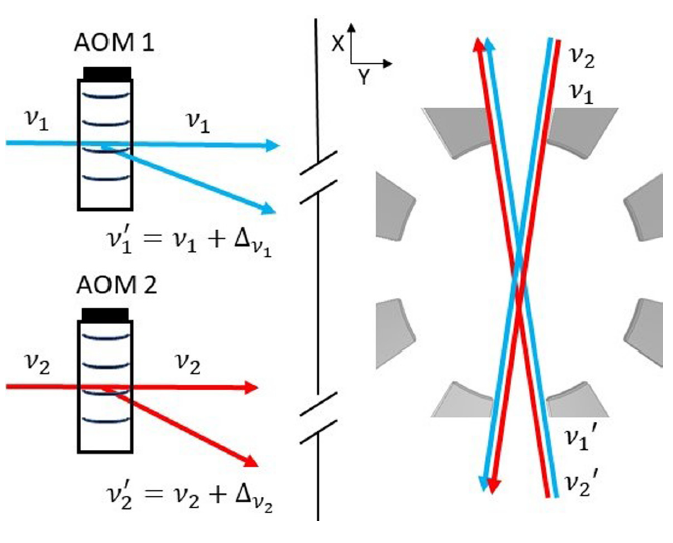
\includegraphics[width=\linewidth]{Kato - Two-tone Doppler cooling of radial two-dimensional cyrstals in a radio-frequency ion trap.png}
    \caption{Two-tone laser-based Doppler cooling. Left, both lasers are divided into two separate beams and one branch of each is passed twice through an acousto-optic modulator (AOM). This generates an additional frequency tone that can be adjusted dynamically without interrupting the original beam. Right, the shifted and unshifted beams are separately combined and then counterpropagated through the segmented ring trap. Borrowed from \textit{Two-tone Doppler cooling of a radial two-dimensional crystals in a radio-frequency ion trap} \cite{Kato}. Description is my own.}
    \label{fig:Two-tone}
\end{figure}

\subsection{Sympathetic Cooling}
I'll briefly touch on another interesting type of cooling known as sympathetic cooling. It's common to see a single ion species used in trapped-ion experiments. However, there are cases when different ions can be combined in "mixed" traps. When this is the case, one ion takes on the role of the "logic" species and the other is the "utility" species. This mixed species setup hopes to avoid some of the problems encountered by single species traps such as decoherence of neighboring ions. One way in which that is accomplished is with sympathetic cooling \cite{Sakrejda}. 

In that situation, the utility ions are used to establish remote entanglement as well as cooling the entire ion chain. The logic ions are then used solely for the quantum information storage and manipulation. In 2020, Sakrejda \textit{et al.} demonstrated an efficient sympathetic cooling scheme using barium (Ba) and ytterbium (Yb) as the utility and logic ions respectively. Sympathetic cooling relies on strong coupling between the logic ions to motional modes because they are only cooled by the collective motion of the chain, while the utility ions are the ones undergoing direct laser cooling. The ordering of ions in the chain will also have a noticeable impact on the motional modes, and in turn, some chain orderings experience better cooling than others \cite{Sakrejda}.